\chapter{Revealing the GeV Supernova Remnant Population}
\label{chap:snrCat}


%\section{Introduction}\label{snrCat:Intro}
\section{\label{snrCat:latGam}Supernova Remnants at \gam~Energies}

By the end of the its science run, \egret{} had detected 271 sources above 100\mev{}, within a minimum detection significance of 4$\sigma$, 170 of which had no clear multiwavelength counterpart, with 81 of those unidentified lying within \blat of the Galactic plane \citep{Hartman99}. The main hindrances to source identification were the numerous potential source counterparts (the \egret{} \psf{} was energy dependent, with a 68\% containment radius of ${\rm \sim 6 ^\circ}$ at 100\mev{} and smaller for higher energies) and the large \egret{} error boxes. In addition to this, the primary method for identifying a \gam{} source as an \snr{} is through a compatible angular extent with  observations at some other wavelength, thus the ability to resolve emission from an \snr{} is vital to understanding the mechanisms therein giving rise to \gam{}s. Figure \ref{fig:3EGSky} shows an \egret{} all-sky map at ${\rm E > 100 \mev}$ where the preponderance of unidentified sources and locations thereof are made clear.  


\begin{figure}[h!]%[t] 
	\centering
	\makebox[\linewidth]{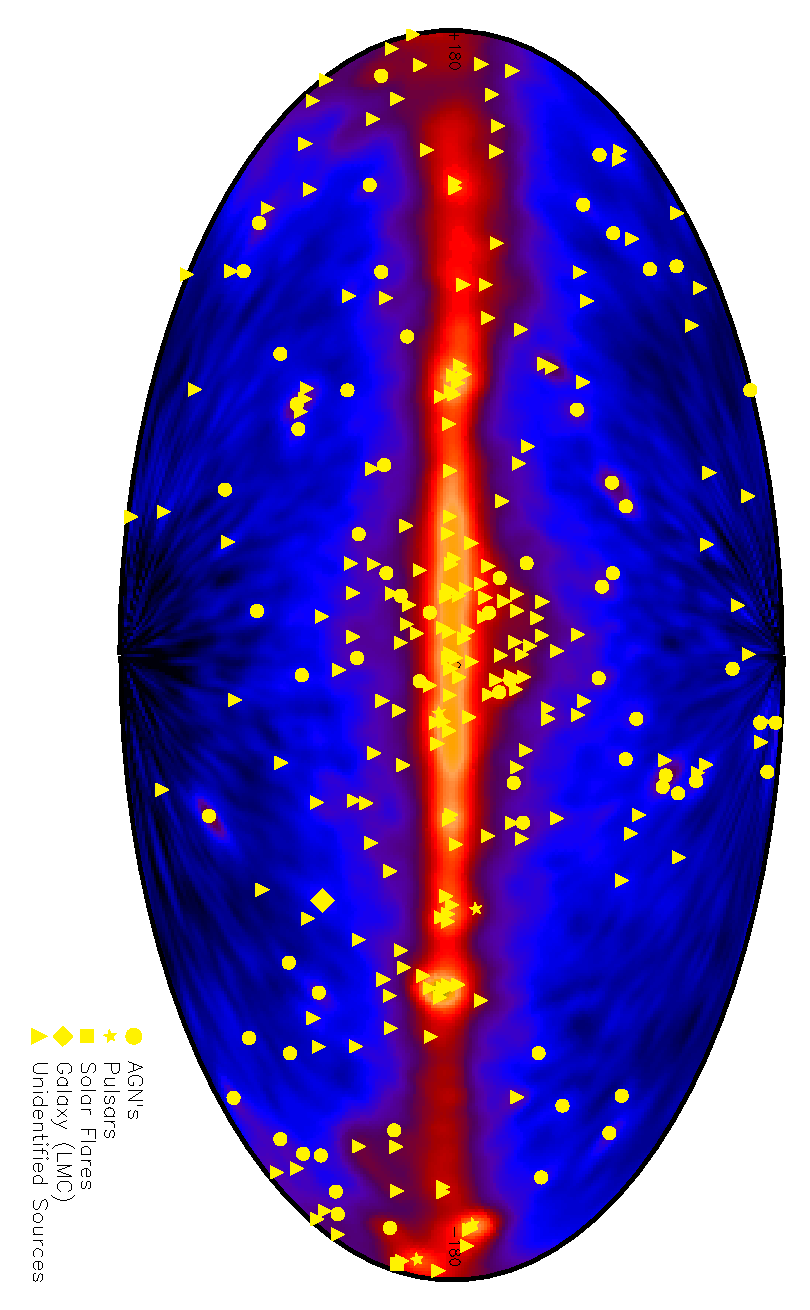
\includegraphics[width=0.8\columnwidth,angle=90]{Figures/3rd_egret_cat.eps} }
	\caption{Third EGRET catalog all-sky map. Unidentified sources represented by triangles. Image courtesy of \url{https://heasarc.gsfc.nasa.gov/docs/cgro/images/epo/gallery/skymaps/}}
	\label{fig:3EGSky} 
\end{figure}

In spite of the difficulties in \egret{} source association, many studies have attempted correlating the unidentified \egret{} sources with various Galactic populations. In particular, several authors found strong evidence for statistical correlation between \glspl{snr} and some of the low-latitude unidentified sources \citep{Sturner95, Esposito96, Romero99}. In a review of the state of potential \snr{} /  \egret{} associations, \cite{Torres03} showed that there were 19 unidentified \egret{} sources that had an \snr~fall within its 95\% error box. Performing Monte Carlo simulations of the population of  \egret~sources, they determined that the chance probability for the 19 sources to be coincident with an \snr~was $1.05 \times 10^{-5}$, implying a probability of 0.99998 that at least one of the associations is real. Despite the statistical correlation of \egret~sources with \glspl{snr}, there were no definitive associations of an \snr~with any \egret~sources.

As the successor to \egret{}, the \lat{} was designed to improve upon its predecessor in a multitude of areas relevant to detecting \snrs{} \citep{atwood09,lat_perf}. The \lat{} has a much improved angular resolution (68\% single-photon containment radius $\sim 0.4^{\circ}$ at 1\gev{} for photons with the best quality direction reconstruction, PSF3 event type, compared to $\sim 1.7^{\circ}$ for \egret{} at the same energy), necessary to resolve \snrs{} as extended objects. The \lat{} also benefits from a superior sensitivity due to a combination of the improved \psf, larger peak effective area ($ {\rm > 9000~cm^2}$ vs. ${\rm \sim 1500~cm^2}$), wider \fov{} (2.4 sr, which is nearly 5 times that of \egret{}), and deeper, more-uniform sky exposure (afforded by the \lat's scanning observations as opposed to \egret's pointing operation). 

This bump in sensitivity results in the \lat{} detecting considerably more sources than \egret. Remarkably, within its first three months of commission, the \lat{} detected 205 sources (above {\rm 10$\sigma$ significance \citep{lat_3m}), and by 11 months, 1451 sources above 4$\sigma$ \citep{1FGL}, compared to  the aforementioned 271 over the entire \egret{} mission. In fact, over its lifetime, \egret{} detected a total of about ${\rm 1.5~x~10^6}$ cosmic photons, while as of March 2016, the \lat{} has detected ${\rm \sim 863~x~10^6}$ source class photons. The \lat's point-source sensitivity peaks between 1 and 10\gev{}, depending on location on the sky. \jamie{plot comparing lat to egret sensitivity?}. With its increased sensitivity and higher energy range (up to $\sim$ 2\tev{} with the recent Pass 8 event reconstruction improvements, which is nearly an order of magnitude higher than \egret{}), the \lat{} is uniquely situated to study the \gam{} morphology and spectra of \snrs{}.

Both energetic lepton interactions (\ie \ic{} radiation of relativistic electrons interacting with ambient photon fields, and nonthermal \brems{}) and hadronic processes ($\pi_0$ decay \gam{}s from \cray{} protons encountering surrounding nuclei) produce spectra observable at \gam{} energies (see Chapter \ref{chap:gamAstr} for details). While the \ic{} generating electron population is also observable through emission of radio \sync{} photons, the proton-proton interaction solely emits \gam{}s. Despite being the prime energy range to observe the effects of cosmic particle acceleration, complexities at the lower \lat{} energy range stymie \snr{} morphology studies.

The \lat{} detects a strong, soft band of diffuse emission in the Galactic plane due to the interactions of  \crs{} with interstellar material. This bright diffuse radiation combined with the multiple potential emission scenarios, broadening \psf{} at decreasing energy, and a high source density in the plane can make it difficult to spatially disentangle sources observed by the \lat{}. To circumvent these 
difficulties, the majority of the analyses undertaken in this thesis are focused on the ${\rm E \geq 1\gev}$ energy range. This energy band is ideal for probing the properties of the accelerated particle populations present in the \snr{} environment. Studies of  \snrs{}  above 1\gev{} benefit from finer \lat{} \psf{}, striking a balance between minimizing the diffuse contribution, maximizing photon sensitivity, and retaining good photon statistics. Furthermore, evolved \snrs{}  exhibit a spectral break between 1-10\gev{}. Explanations for the break range from Alfv\' en wave evanescence generated by collisions of partially ionized material in \mcs{} overtaken by \snr{}  shocks \citep{Malkov11}, reflected shocks in clouds \cite{Inoue10c}, and energy-dependent diffusion from shocks \cite{Ohira11}. Studying \snrs{} in this energy range hones our capability to tackle several goals set out by the \Fermi{} team when the mission was conceived.

Two of the primary science goals of the \lat{}  are to 1. resolve the \gam~sky, uncovering the nature of the unidentified sources detected by \egret{}, and 2. to understand the mechanisms of cosmic particle acceleration \citep{atwood09}. In this chapter, we describe our efforts towards addressing these questions by studying the \gam{} emission coincident with sources comprising the population of known radio emitting \snrs{}.

Prior to this work, several individual studies with the \lat{} had successfully resolved spatially extended emission from \snrs{} \citep[and references therein]{3FGL}, yet no systematic analysis leveraging the \lat{}'s full-sky coverage had yet been performed. We performed a uniform study of the \snrs{} in aggregate to measure the properties common to these objects. An understanding of these common characteristics allows us to assess \snrs{} as a class of \gam{} and \cray{} emitting objects and serves as the impetus for this uniform analysis of the known Galactic \snrs{}. We  report here on the published results from the \snrcat{} \cite{SNRcat}. \jamie{they aren't published yet, but almost maybe that will change by June}
 
 \jamie{2FGL only had 7 ID'd SNR, 4 snr, 58 spp. 3FGL had 12 SNR, 11 snr, 49 spp. I'm not sure what made some snr vs. spp. They must have all been point sources right? No known radio pwn, psr?}

\section{\label{snrCat:ptlk}The \ptlike~  Maximum Likelihood Package}

This section is about the tools (and intricacies there in) developed to study SNRs with Fermi

Describe pointlike and what problems it aims to solve in contrast to gtlike.

pointlike is good at analysis where iteration is key because it takes some shortcuts with some integrals and is faster than gtlike. 

Not sure how much to talk about pointlike here vs. modifiying what's in the next chapter from the snrcat paper. 

The addSrcs framework extends/exploits pointlike 

addSrcs in this section or merged into the next one?

I need to stress that this is not just a tool developed, but there's an art and finesse to it (talk about the problems we overcame), there was much iteration.

tool plus knowledge to get the best result

what are the aspects of addSrcs tht needed knowhow, finagling

\jamie{the following  is from a confluence page motivating and describing  addSrcs}

To attain the best understanding of a source of interest, the best characterization of the corresponding ROI is necessary. This is particularly challenging in dense source and strong diffuse dominated regions (i.e. the Galactic plane). We have developed an automated method for systematically locating and modeling all potential point and/or extended sources in an \roi{} using \ptlike{}. This work started as a parallel and complementary analysis to the SNR cat pipeline, intended to minimize possible bias introduced by the initial model for an ROI (e.g 2FGL) It is  used to derive the input sources model for the SNR catalog. The goal of this work is to use this "add sources" method to aid in characterization of GeV emission near SNRs and nearby molecular clouds.

what are some motivations for various addSrcs decisions 

How to distinguish addSrcs from how addSrcs was applied to the SNR cat. For the SNRcat, it was addSrcs in PS mode with specifics relevant to the SNR cat needs (like what?)


Describe how we put together/designed this analysis what questions were we trying to answer?


tested pipeline with 6 sources (I have the tests somewhere, see old Fermi symp poster, Gal Evo too)
\section{Input Source Model Construction}\label{snrCat:AddSrcs}

\jamie{add some more bkg on the SNR cat here and add more of the snrCat intro}


To characterize each candidate SNR we constructed a %n optimal 
model of \g-ray emission in the RoI which includes all significant sources of emission as well as the residual background from CRs misclassified as \g-rays. We implemented an analysis method to create and optimize the \jamie{fill this in }~models for each of the 279 RoIs. For each RoI, we started with all sources listed in 
%We started with a list of cataloged sources within our RoI from 
the \twofgl \citep{2FGL}, based on $2$\,years of Source class data, within the RoI. To this we add pulsars from \twopc \citep{2PC}, based on $3$\,years of source class data, with 2PC taking precedence for sources that exist in both. 
For the diffuse emission we combined the standard IEM corresponding to our P7 data set, gal\_2yearp7v6\_v0.fits, with the standard %. To this we added a 
model for isotropic emission, which accounts for extragalactic diffuse \g-ray emission and residual charged particles misclassified as \g-rays. 
%We used the standard IEM corresponding to our P7 data set, gal\_2yearp7v6\_v0.fits, and the 
Both the corresponding isotropic model, iso\_p7v6source.txt, and the IEM are the same as used for the 2FGL catalog analysis\footnote{Further details on the diffuse emission models are available at \url{http://fermi.gsfc.nasa.gov/ssc/data/access/lat/BackgroundModels.html}}.
% Files used are equivalent to FSSC models: ring_2year_P76_v0.fits, isotrop_2year_P76_source_v0.txt

%To better optimize our model, 
Compared to 2FGL, we used an additional year of data and limited the energy range to $1-100$\,GeV. This can result in different detection significances and localizations than previously reported in 2FGL. To account for these effects, we recreated the RoIs' inner $3$\degr{}\,radius regions, which encompass the radio extents of all known SNRs, observed to be $\leq 2.6$\degr{} and allows a margin for the LAT PSF. 
The weighted average $68\%$~containment radius of the LAT PSF for %front and back converting 
events at $1$\,GeV is $\sim0.7$\degr{} \citep{lat_cm}. 
We note that this implicitly assumes that an SNR's GeV extent should not be more than about an order of magnitude larger than its radio extension and also note that the selection biases stated in Green's catalog limit the range of known SNRs' radio extensions. 

To build the inner $3$\degr{}\,radius model of each RoI, we first removed all sources except identified Active Galactic Nuclei (AGN) and pulsars, whose positions on the sky are independently confirmed by precise timing measurements \citep{2PC}. Retained AGN were assigned their 2FGL positions and spectral model forms. Pulsars' positions and spectral forms were taken from 2PC. 2FGL sources identified or associated with SNRs are removed when they lie within the inner $3$\degr{}. %The removal included SNRs included in 2FGL. 

We generated a map of source test statistic (TS) defined in \citet{Mattox96} via \ptlike{} on a square grid with $0.1$\degr{}\,$\times$\,$0.1$\degr{} spacing that covers the entire RoI. \ptlike{} employs a binned maximum likelihood method. The source TS is defined as twice the logarithm of the ratio between the likelihood~$\mathcal{L}_1$, here obtained by fitting the model to the data including a test source, and the likelihood~$\mathcal{L}_0$, obtained here by fitting without the source, i.e., $\textrm{TS = 2 log}(\mathcal{L}_1/\mathcal{L}_0$). At the position of the maximum TS value, we added a new point source with a Power Law (PL) spectral model:
%\terri{\g{} is implicitly negative here but is used as positive everywhere in the pipeline and following plots. Verify that setting to explicitly positive here works for sections between here and pipeline results.} \jack{done.}
\begin{equation}
	\label{eqn:PL}
	\frac{dN}{dE} = N\frac{(-\Gamma+1)E^{-\Gamma}} {E_{\rm max}^{-\Gamma+1} - E_{\rm min}^{-\Gamma+1}}
\end{equation}
where $N$ is the integrated photon flux, $\Gamma$ is the photon index, and $E_{\rm min}$ and $E_{\rm max}$ are the lower and upper limit of the energy range in the fit, set to $1$\,GeV and $100$\,GeV, respectively.
We then performed a maximum likelihood fit of the RoI to determine $N$ and $\Gamma$ and localized the newly added source. 
The significance of a point source with a PL spectral model is determined by the $\chi^2_n$ distribution for $n$ additional degrees of freedom for the additional point source, which is typically slightly less than~$\sqrt{\textrm{TS}}$\footnote{See \url{http://fermi.gsfc.nasa.gov/ssc/data/analysis/documentation/Cicerone/Cicerone_Likelihood/TS_Maps.html} for further details.}.

To promote consistent convergence of the likelihood fit, we limited the number of free parameters in the model. For sources remaining after the removal step, described above, we freed the normalization parameters for the sources within $5$\degr{} of the RoI center, including identified AGN and pulsars. For 2FGL sources between $5$\degr{} and $10$\degr{}, we fixed all parameters. The spectrum of the IEM was scaled with a PL whose normalization and index were free, as done in 2FGL.
%\terri{why is this reference here?} \jack{same as done in 2FGL}. 
For the isotropic emission model, we left the normalization fixed to the global fit value since the RoIs are too small to allow fitting %separately fit 
the isotropic and Galactic IEM components independently. The isotropic component's contribution to the total flux is small compared to the IEM's at low Galactic latitudes.

After localizing them, the new sources were tested for spectral curvature. In each of the $4$~energy bands per decade we calculated the TS value for a PL with spectral index fixed to $2$ and then summed the TS values. 
%We summed TS values for fits in individual energy bands, each calculated in an energy band for a PL model of fixed spectral index~$2$, with $4$~energy bands per decade. 
We refer to this as $\mathrm{TS_{band fits}}$. A value for $\mathrm{TS_{band fits}}$ much greater than the TS calculated with a PL ($\mathrm{TS_{PL}}$) suggests with a more rapid calculation that the PL model may not accurately describe the source. %, where $\mathrm{TS_{PL}}$ is the TS with a PL fit. 
Analogously to 2FGL \citep{2FGL}, we allow for deviations of source spectra from a PL form by modeling sources with a log-normal model known colloquially as LogParabola or logP:
\begin{equation}
	\newcommand{\pfrac}[2]{\left(\frac{#1}{#2}\right)} \frac{dN}{dE} = N_0\pfrac{E}{E_b}^{-(\alpha + \beta\log(E/E_b))}
	\label{eqn:logP}
\end{equation}
where $N_0$ is the normalization in units of photons/MeV, $\alpha$ and $\beta$ define the curved spectrum, and $E_b$ is fixed to $2$\,GeV. If $\mathrm{TS_{band fits} - TS_{PL}} \geq 25$, we replaced the PL spectral model with a logP model and refit the RoI, including a new localization step for the source. We retained the logP model for the source if the global \logL{} across the full band improved sufficiently: 
$\mathrm{TS_{curve}} \equiv 2 ($\logL{}$_{\mathrm{logP}}-$\logL{}$_{\mathrm{PL}}) \geq 16$. 
Otherwise we returned the source to the PL model which provided the better global \logL. Across all RoIs, less than $2\%$ of the newly added sources retained the logP model. 

We continued iteratively generating TS maps and adding sources within the entire RoI until additional new sources did not significantly change the global likelihood of the fit. The threshold criterion was defined as obtaining $\mathrm{TS < 16}$ for three consecutively added new sources, denoted as $\mathrm{N_{TS < 16} = 3}$. Despite iteratively adding a source at the location of the peak position in the TS map, the TS values of new sources may not decrease monotonically with iteration for several reasons. First, source positions were localized after fitting the RoI and generating the TS map. Second, some added sources were fit with a more complex spectral model than a simple PL. Finally, when creating the TS map, we fixed the source's spectral index to $2$, whereas when adding the actual source to the model, we allowed its index to vary. 

The specific value of $\mathrm{N_{TS < 16} = 3}$ was chosen to avoid missing sources with $\mathrm{TS \geq 25}$, the threshold commonly used for source detection in LAT data, and to optimize computation time. We tested the threshold by selecting eight representative SNRs from both complex and relatively simple regions of the sky, with both hard and soft spectral indices. We applied the above procedure to the test RoIs using a criterion of $\mathrm{N_{TS < 16} = 6}$ and counted how many $\mathrm{TS \geq 25}$ sources would be excluded if a smaller $\mathrm{N_{TS < 16}}$ criterion was used. Reducing the threshold to $\mathrm{N_{TS < 16} = 3}$ cut only one significant source in any of the regions. Since the maximum number of sources added in any test RoI was $38$, the minimum $14$, and the total number of sources added across all test regions was $221$, we chose to use $\mathrm{N_{TS < 16} = 3}$ for the full sample. To allow for proper convergence of the likelihood fit, we reduced the number of free parameters prior to each new source addition. If the previously added source was between $3$\degr{} and $5$\degr{} of the center of the RoI, just its normalization was freed, and if greater than $5$\degr{} all its source parameters were fixed.

To avoid having newly added sources overlap with pulsars, we deleted new sources from the RoI if they were within~$0.2$\degr{} of a \g-ray pulsar and refit the pulsar in the $1-100$\,GeV range following the 2PC conventions. 
2PC modeled pulsar spectra as PL with an exponential cutoff (PLEC),
\begin{equation}
	\newcommand{\pfrac}[2]{\left(\frac{#1}{#2}\right)} \frac{dN}{dE} = N_0 \pfrac{E}{E_0}^{-\Gamma} \exp\left(-\frac{E}{E_c}\right)^{b},
	\label{eqn:PLEC}
\end{equation}
where \textit{$N_0$} is the normalization factor, \textit{$\Gamma$} is the photon spectral index, \textit{$E_c$} the cutoff energy, and $b$ determines to the sharpness of the cutoff. 2PC assessed the validity of fixing $b$ to $1$ in Equation~\ref{eqn:PLEC} (PLEC1) 
%Fixing $b$ in Equation \ref{eqn:PLEC} to $1$ (PLEC1),  the PLEC1 model, 
by repeating the analysis using a PL model, as well as the more general exponentially cut off PL form, allowing the parameter $b$ in Equation~\ref{eqn:PLEC} to vary. For the pulsar spectra in this analysis, we compared the maximum likelihood values for spectral models with and without a cutoff and with and without the value of $b$ being free, via %model's likelihoods as: 
$\mathrm{TS_{cut}} \equiv 2 ($\logL{}$_{\mathrm{PLEC1}}-$\logL{}$_{\mathrm{PL}})$ and $\mathrm{TS}_{b} \equiv 2 ($\logL{}$_{\mathrm{PLEC}}-$\logL{}$_{\mathrm{PLEC1}})$ to determine which to use. If $\mathrm{TS_{cut}} < 9$ is reported for the pulsar in 2PC then a PL model is used. If TS$_{\mathrm cut} \geq 9$, we then check to see if the cutoff energy fit in 2PC lies within the restricted energy range of $1-100$\,GeV used in this work. For pulsars with cutoffs $\geq 1$\,GeV, we then use the PLEC model if TS$_{\mathrm b} \geq 9$, and the PLEC model with cutoff freed otherwise. %\terri{This says you use the free b PLEC regardless of $\mathrm{TS}_{b}$'s value, which can't be right.} 
For those pulsars with cutoffs less than 1 GeV the spectral parameters are fixed to the 2PC values.

%\[ \begin{dcases*}
%        \mathrm{PLEC} & if TS$_{\mathrm b} \geq 9$ \\
%        \mathrm{PLEC1} & if TS$_{\mathrm b} < 9$ and TS$_\mathrm{cut} \geq 9$ \\
%        \mathrm{PL} & if TS$_\mathrm{cut} < 9$
%        \end{dcases*}
%\]
%\terri{Jamie (Jack?), please verify this. NB: I derived this from the text (now in comments) and there are cases oddly covered here, e.g. of TS$_{\mathrm b} \geq 9$ \&\& TS$_\mathrm{cut} < 9$ is nominally doubly specified as both PLEC and PL, while TS$_{\mathrm b} < 9$ \&\& TS$_\mathrm{cut}  < 9$ seems to be both a PLEC1 and a PL).}
%\jack{This is what was done in addSrcs, but not what was done in the pipeline, where I had to explicitly add in the 2PC pulsar results as the first step in the model. Text has been re-written to reflect how pulsars are handled in the pipeline using 2PC.}

% a PLEC model for a pulsar if $\mathrm{TS_{b}} \equiv 2 ($\logL{}$_{\mathrm{PLEC}}-$\logL{}$_{\mathrm{PLEC1}}) \geq 9$,
%%%$\mathrm{TS_{b} \equiv 2\Delta log( likelihood) \geq  9}$between PLEC1 and PLEC,
%PLEC1 if $TS_{b} < 9$ 
%\[  
% \mathrm{TS_{cut}} \equiv 2(\log \mathcal{L}_{\mathrm{PLEC1}}-\log \mathcal{L}_{\mathrm{PL}}) \begin{dcases*}
%        \mathrm{PLEC1} & if TS$_{cut} \geq 9$ \\
%         \mathrm{PL} & if TS$_{cut} < 9$
%        \end{dcases*}
%\]
%and $\mathrm{TS_{cut}} \equiv 2 ($\logL{}$_{\mathrm{PLEC1}}-$\logL{}$_{\mathrm{PL}}) \geq 9$
%%$\mathrm{TS_{cut} = \Delta log(likelihood) \geq 9}$ between PLEC1 and PL,
%, and finally, if $\mathrm{TS_{cut} < 9}$ we used a PL spectral model. 

To complete the construction of our point source RoI model, we took the output of the previous steps and removed all sources with TS~$< 16$. This final model was then used as the starting model for analyzing candidate SNR emission. We conservatively allow sources with TS down to $16$ $(\sim4\,\sigma)$ in order to account for the effects of at least the brightest sub-threshold sources on the parameter fits for the other sources in the model. Furthermore, while the SNR analysis method described in the next subsection (\ref{Sec:DetectMethod}) is allowed to remove sources, it cannot add them. Thus we start from a set of sources designed to allow the final model to capture all significant emission within the central region. To corroborate our method of systematically adding sources to a region, we compare our RoI source models with those found by the 2FGL approach in Appendix~\ref{appen:addSrcs2FGL}. 


\section{Comparison of Source Models with 2FGL}
\label{snrcat:addSrcs2FGL}

This SNR catalog was constructed using $3$~years of P7 Source class data in the energy range $1-100$\,GeV, whereas 2FGL used $2$\,years of data over the larger energy range $0.1-100$\,GeV. The differences in observing time and energy range resulted in residual, unmodeled emission in some RoIs as well as changes to some 2FGL sources' spectral model, position localization, and detection significance. Here we compare the input source models constructed for this catalog, described in Section~\ref{Sec:AddSrcs}, with 2FGL to better understand the method's ability to describe the regions studied. Since we rederive the input source model only within a $3\degr$\,radius of the center of each RoI, 
%removed from our source model all 2FGL sources within a $3\degr$\,radius of the center of each RoI except those identified as AGN and pulsars, 
we consider sources only inside that radius.

Given the data set differences, in each RoI we expect similar but not identical numbers of sources relative to those in 2FGL.
Figures~\ref{fig:2FGLvAddSrcs} and \ref{fig:2FGLvAddSrcsAssoc} show the numbers of significant (TS\,$\geq 25$) 2FGL sources and derived input model sources (excluding 2FGL identified AGN and pulsars kept in the input model) in individual RoIs as 2D histograms. In Figure~\ref{fig:2FGLvAddSrcs}, 
the number of sources in the derived input model is typically greater than the number of 2FGL sources that are significant at $1-100$\,GeV. 73 of the 279 RoIs studied contain at least one of the the 12 extended 2FGL sources. Since 2FGL extended sources were removed from the inner $3\degr$ of each RoI, and this region was repopulated with point sources, we can detect multiple point sources inside the extent of any removed extended 2FGL sources. This decomposition of extended sources, combined with the longer data set and different energy range compared to 2FGL, contribute to the high ratio of input model to 2FGL sources in some RoI, which demonstrates the need to rederive the source model. %Included among these newly added sources are sources that may not be coincident with a 2FGL source. 

\begin{figure}[h!]
	\centering
	\makebox[\linewidth]{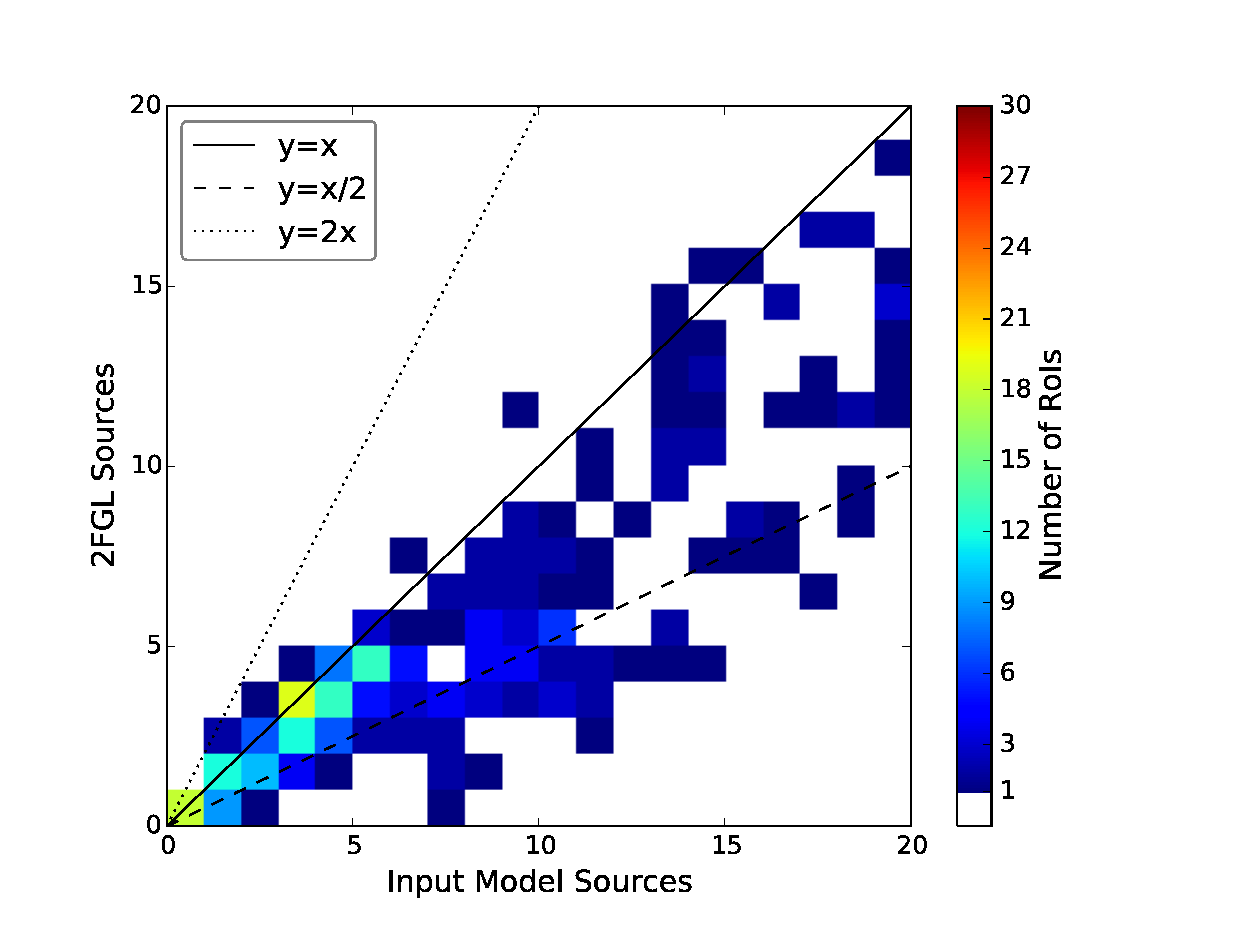
\includegraphics[width=0.8\columnwidth]{figures/addSrcs_2FGLnoAGNPSR_TSgt25_in3deg_2dhist_maj.eps} } 
	\caption{Comparison of the number of 2FGL sources with TS$_{1-100\,\mathrm{GeV}} \geq 25$ (excluding AGN and pulsars) with the number of newly added input model sources in the present analysis, for sources within $3$\degr{} of the center of each RoI. The color scale shows the number of RoIs with a particular combination of numbers of 2FGL sources and new sources.
		%The color scale shows the number of RoIs with a particular ratio of 2FGL to new sources. 
		White corresponds to no RoI with that combination of source counts.}
	%\terri{We are exploring the reasons why there could be more or fewer sources of a given type in an RoI. For instance, multiple addSrcs sources could be associating to the same 2FGL source. There are also cases where the added source is close by not quite within  $0.2$\,\degr{} of the 2FGL source.}
	\label{fig:2FGLvAddSrcs} 
\end{figure}

To more accurately represent the 2FGL sources being reproduced in the central $3\degr$, in Figure~\ref{fig:2FGLvAddSrcsAssoc} we limited the input model sources to those within $0.2\degr$ (approximately the width of the core of the $10$\,GeV PSF) of a 2FGL source, effectively excluding input sources that are not co-spatial with a 2FGL source. Here we see that the majority of 2FGL sources have counterparts in the rederived set. 
As a region's complexity increases, seen as an increase in numbers of 2FGL sources, up to about half of the 2FGL sources may not have counterparts within $0.2$\degr. Given that in these same regions we have more new sources than 2FGL sources, as seen in Figure~\ref{fig:2FGLvAddSrcs}, we find as expected that the longer data set with improved statistics at higher energies, where the angular resolution of the LAT is the best, allows us to add new sources to account for newly significant excesses in these complex regions. 
%As mentioned above, we do not expect to precisely reproduce the results of 2FGL. 
Additionally, sources with low TS in 2FGL are particularly susceptible to having a newly added source which may start at a similar position but then localize further than $0.2\degr$ from the 2FGL source. 

Thus, we find that the method developed and used here produces a model which reproduces the 2FGL sources as expected, including differences that trend as anticipated given the longer data set and modified energy range, yielding better spatial resolution. The new method thus provides reasonable representations of the regions being modeled as input for the final analysis.

%\terri{Suggest removing (the remainder of) this paragraph.} 
%Additional discrepancies between our source model and 2FGL can arise from shifting of source position of low TS 2FGL sources \terri{2FGL sources can't shift positions...} (i.e. newly added sources separated from a 2FGL source by more than $0.2\degr$, particularly sources with high flux neighbors), and association of 2FGL sources with newly added sources outside $3\degr$ (and vice versa) \terri{Per Section~\ref{Sec:AddSrcs}, we're not removing or adding sources outside $3\degr$, so why is this the case?}. Despite this, Figure \ref{fig:2FGLvAddSrcsAssoc} shows that in many RoI, our source model recovered most of the 2FGL sources.


% % %
\begin{figure}[h!]%[t] 
	\centering
	\makebox[\linewidth]{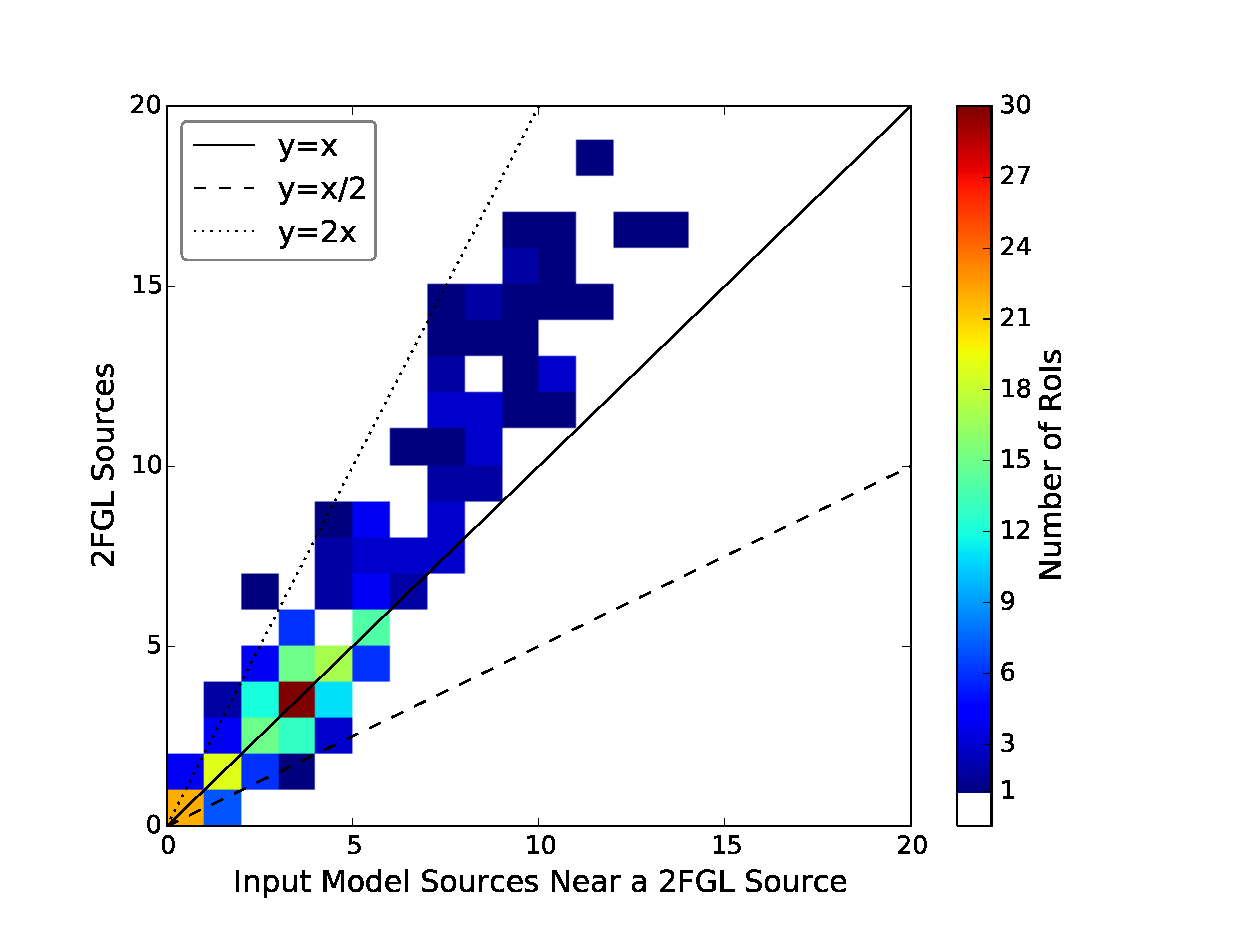
\includegraphics[width=0.8\columnwidth]{figures/addSrcsWassoc_2FGLnoAGNPSR_TSgt25_in3deg_2dhist_maj.eps} }
	\caption{Same as Figure~\ref{fig:2FGLvAddSrcs}, including only input model sources lying within $0.2$\degr{} of a 2FGL source.}% within $3$\degr{} of the center of an RoI and with TS$_{1-100\,\mathrm{GeV}} \geq 16$, .}
	\label{fig:2FGLvAddSrcsAssoc} 
\end{figure}
% % %

\section{SNR Catalog Results}
\label{snrCat:results}
What to include from SNR cat

Pull parts of the intro/abstract as needed.

sections: 2, 2.1, 2.2, 2.3 (do I need 2.3.1, 2.3.2)

 First par of 3.1 about how we classify. Summarize some of the relevant catalog results of section 3.2. There's no real reason to include the catalog tables I think. Parts of 3.2.1 3.2.2, 3.2.3 just to highlight which sources were newly detected. 
 
 What to include from section 4? I didn't make these plots, but I contributed to the pipeline script and gave advice on things. 
 
 For the mock snrCatalog, I didn't do the analysis, but I ran addSrcs on the mock sources. maybe there's not much to say about this though.

Section 5? It's not my work, but I participated in discussions, edited text in the section a little bit. I think something needs to be included from this because one of the points of the paper was to see what we could say about the total energy in CR in the Galaxy

Parts of conclusion

Which figure to include from snr cat results?


\section{Summary}\label{snrCat:summ}
In this chapter, we have presented results from the publication of the \snrcat. Application of addSrcs adding point sources to characterize emission in an\roi. Give more details on validation and testing than was given in the paper, as well as details on the code. Work on fitting single extended source, present some work on detected SNRs and population properties, implications for total power in cosmic rays (don't focus on this because it wasn't where I contribute the most). Mock catalog contributions. Testing with extended sources or don't mention too much because we decide not to apply it here?

With its unprecedented sensitivity and angular resolution above 1\gev, the \lat~provides for the first time the opportunity to distinguish SNR-emitted photons from their backgrounds, and  to unambiguously detect and identify dozens of \glspl{snr}. \jamie{maybe this is for the intro/abstract because it's a little vague}

The \lat{} is uniquely situated to address these goals and definitively detect and identify dozens \snrs

Focus our efforts on
\section{Scratch}
has the spatial and spectral sensitivity to resolve

good spatial and spectral 


talk about how much "power" comes from the higher energy  range,

EGRET point source sensitivity is ${\rm \sim1x10^{-7}}\flux{}$
 \url{http://fermi.gsfc.nasa.gov/science/instruments/table1-1.html} get this number from somewhere else


\jamie{somewhere I should also say that identifying an extended source as such gives better spectra, see 2FHL}

\cite{Thomson93}, egret observed a total of 1.5 million celestial \gam{}

\jamie{ Fermi goals: 1. Resolve the \gam~sky: the origins of diffuse emission and the nature of unidentified sources: Source identification through good source localization, measurement of spectra across broad energy range, nearly continuous monitoring of the sky for temporal variability
	2. Understand the mechanisms of particle acceleration in celestial sources:}

\jamie{understanding accel plus identification of the potential SNRs motivates the SNR cat }

\jamie{snrs as source of Galactic cosmic rays, and thus as drivers of Galactic evolution}

-what's to gain from studyng the population vs individual?

-constraint on CR energy density in the Galaxy

-do the observed g-ray properties match those
of models?

-like index etc?